\chapter{Final Design Overview}\label{chapter:finaldesign}
The overall exergame development was user centered. Based on the feedback gathered from the prototype game review, discussions with experts, new movements have been introduces and modifications have been made to the existing design in order to make the exergame more engaging, enjoyable, and intuitive to use for the future users. This section outlines the design and development of the final version of the Immotion exergame for warm up routine guidance and motivation.
\section{A Modular Design Approach}
In order to make the exergame easily adjustable for user requirements we followed a modular design approach. That is, each movement (exercise) that is required from the user to be performed is represented by one distinct game segment. To put it differently, the whole game system was subdivided into smaller parts, that could be independently created and then used accordingly. That way, by combining multiple segments randomly, we were able to generate a unique game map each time the user played the exergame. The game is not constrained by one global map, but a dynamic one created on each game run. Moreover, having segments as the basic game artifacts, allowed us to easily add new segments that make the game richer and the set of required movements bigger. Also, this way we easily discarded segments and movements users disliked or were difficult to perform. We believe this is a major feature that makes the our exergame scalable and extensible for future user requirements and preferences. 
\section{Home Window Overview}
When the user starts the exergame, the \textit{Home screen} that is depicted in Figure \ref{fig:start} is showed. Apart from starting the game, other options are available to the user. The user can then chose from the following options:
\begin{itemize}
\item Start
\item Help
\item Volume
\item High Score
\item Quit
\end{itemize}
\begin{figure}[h]
    \centering
    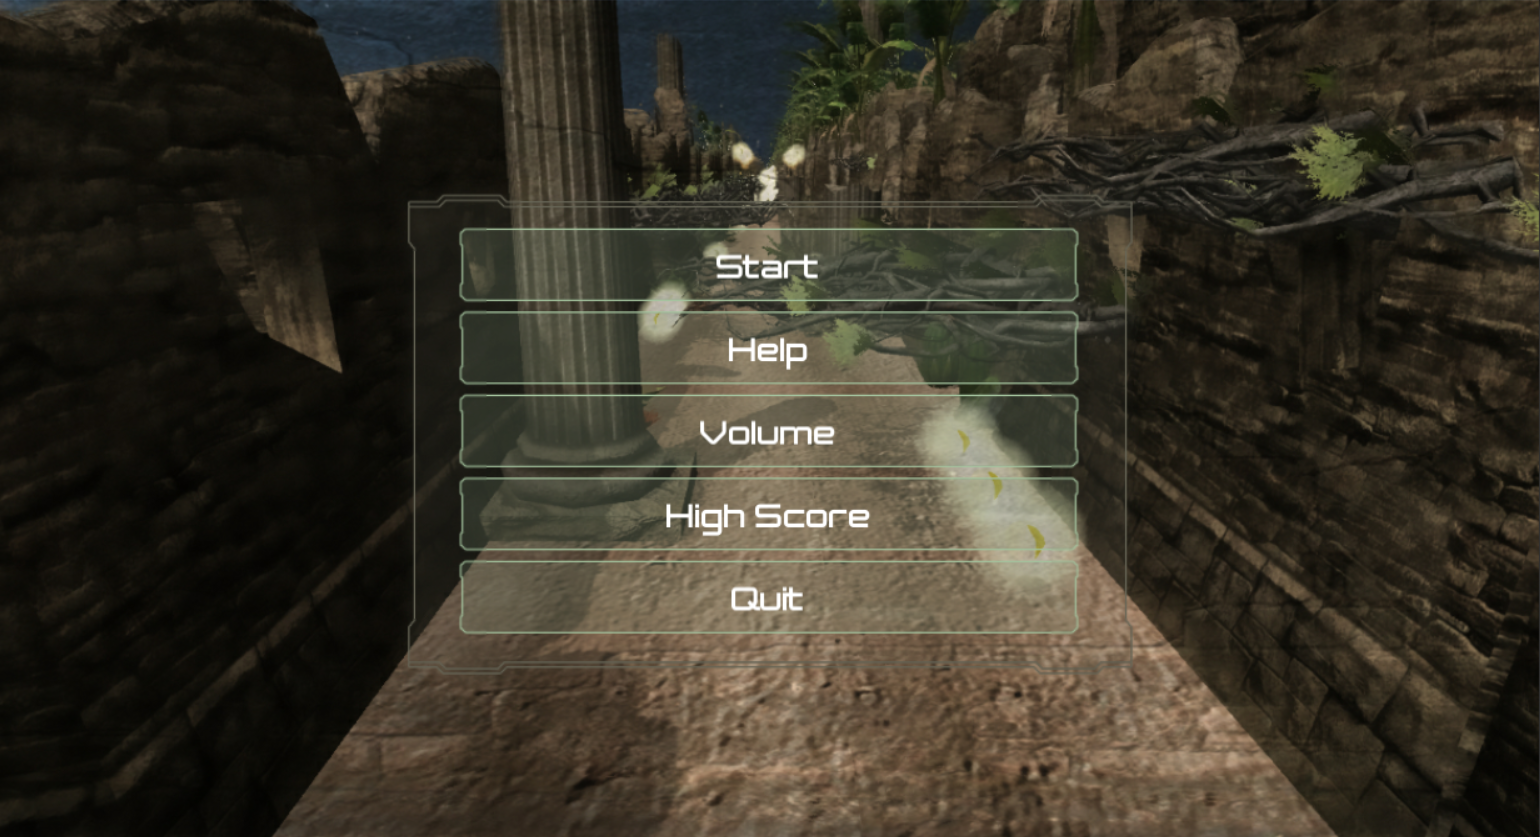
\includegraphics[width=\textwidth]{Start}
    \caption{Home screen.}
    \label{fig:start}
\end{figure}
Next, the above listed options will be further detailed.\pagebreak
\paragraph{Start Menu}
By selecting the Start button, the user is presented with a new screen showed in Figure \ref{fig:userinfo} where user input is required.\\
\begin{figure}[h]
    \centering
    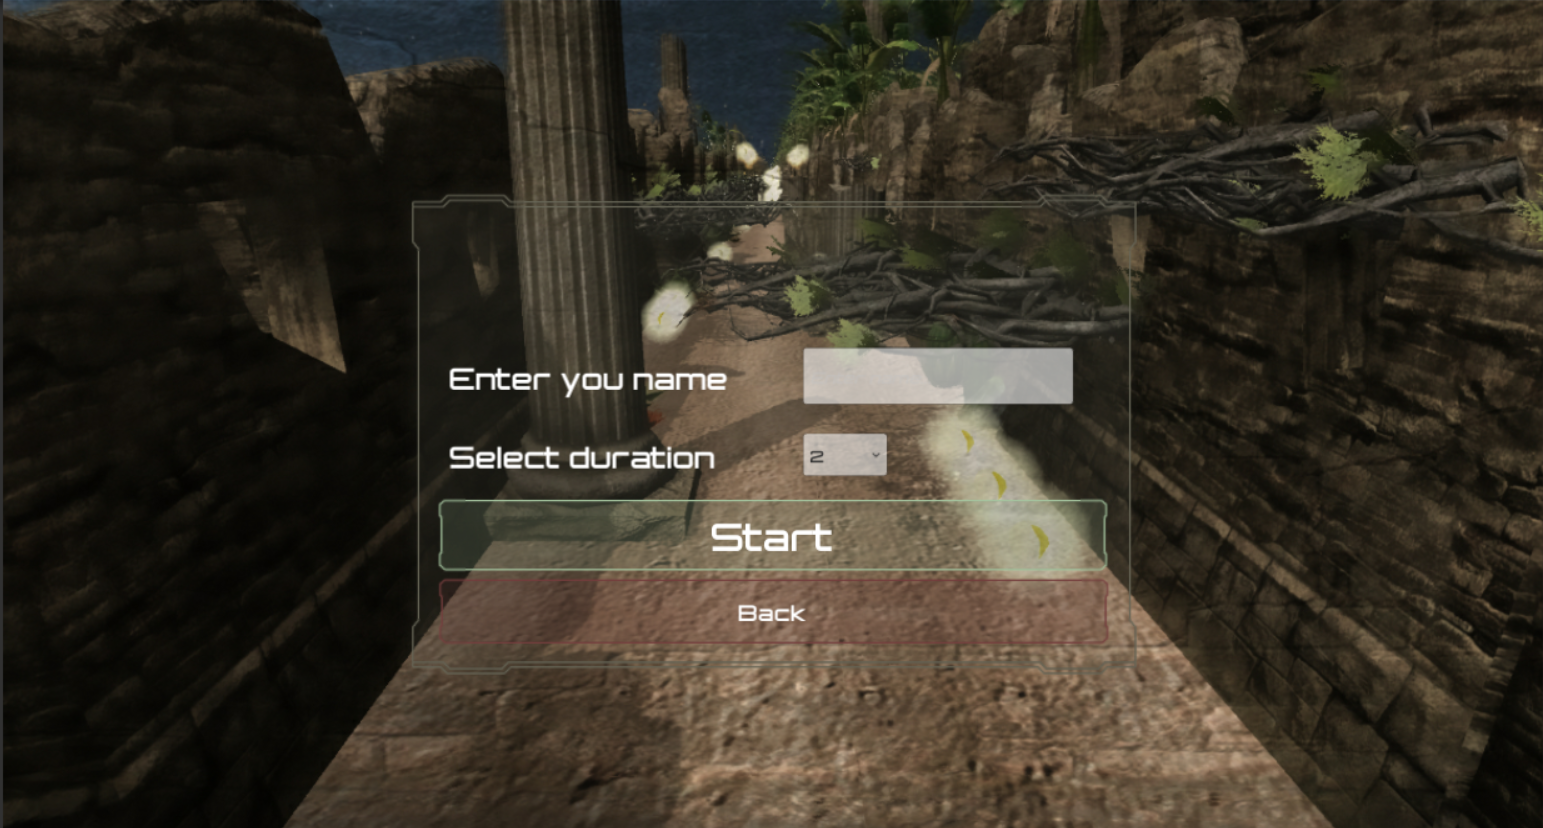
\includegraphics[width=\textwidth]{EnterName}
    \caption{User Info Menu.}
    \label{fig:userinfo}
\end{figure}\\
For the purpose of tracking users' progress over time and their achievements, we asked them to input their name or username they would like to use in during the gameplay. Based on the username, we displayed users current and highest scores in the Individual score board showed in Figure \ref{fig:individualScore}. After the user set the username and clicked on the Start button, a countdown screen as displayed in Figure \ref{fig:counter} was first presented. The countdown was set to 5 seconds. We opted for this duration because it showed as the most optimal in our pilot study previously conducted with the university personal. This amount of time was sufficient for the test players to prepare for the upcoming exercise by moving to the correct position. In case the user was not in the Kinect sensor range at the beginning of the game, a popup screen informed the user about this. Also, this screen was shown in case the connection to the Kinect sensor failed. The info screen is presented in Figure \ref{fig:witing}. By selecting the \textit{Back} button, the user can go back to the previous Home screen.\pagebreak
\begin{figure}[h]
    \centering
    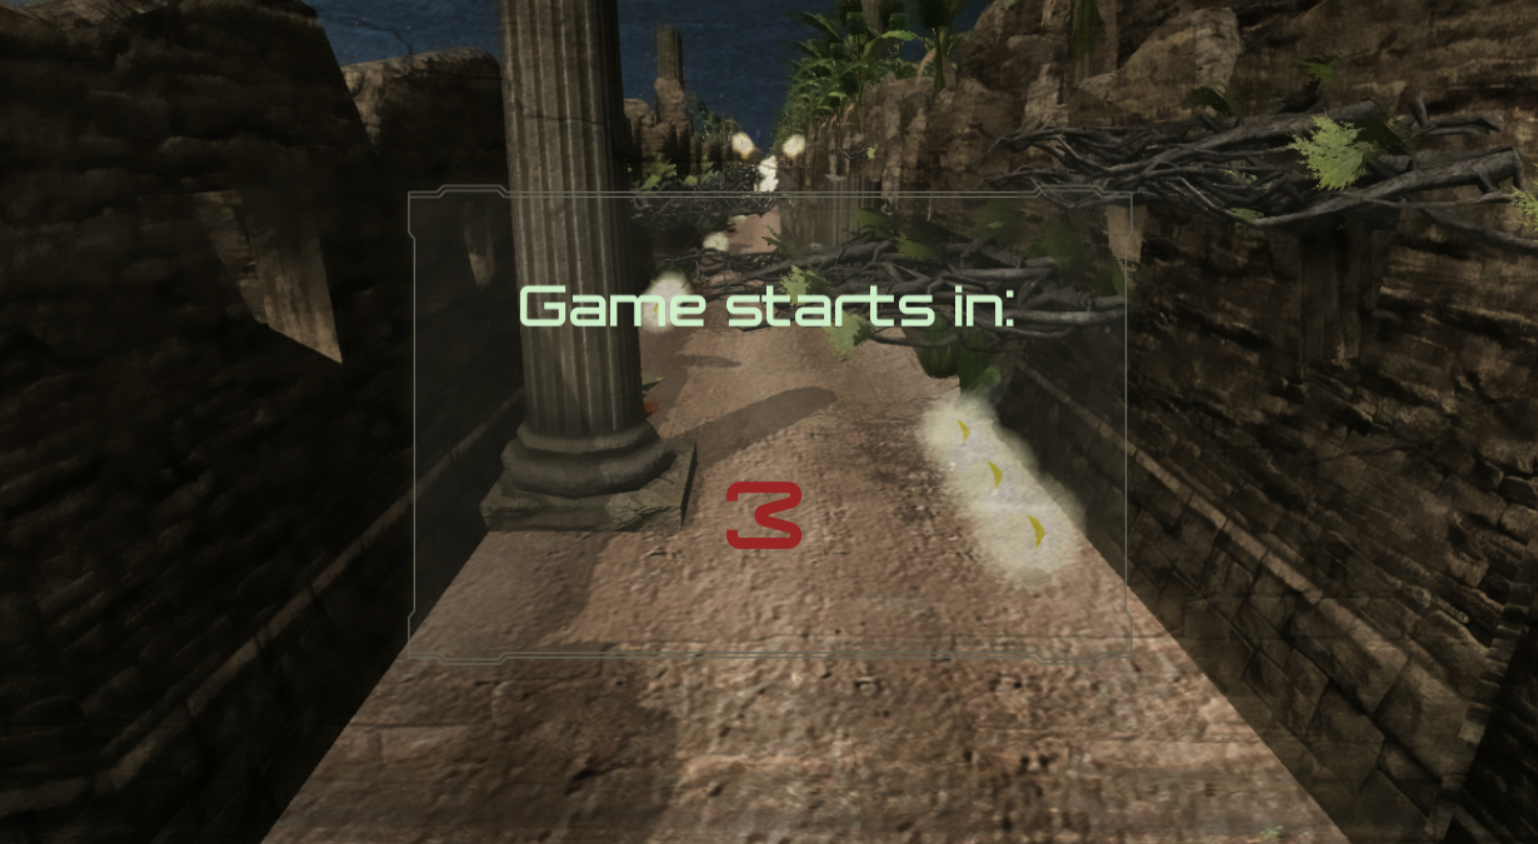
\includegraphics[width=\textwidth]{Counter}
    \caption{Countdown screen.}
    \label{fig:counter}
\end{figure}
\begin{figure}[h]
    \centering
    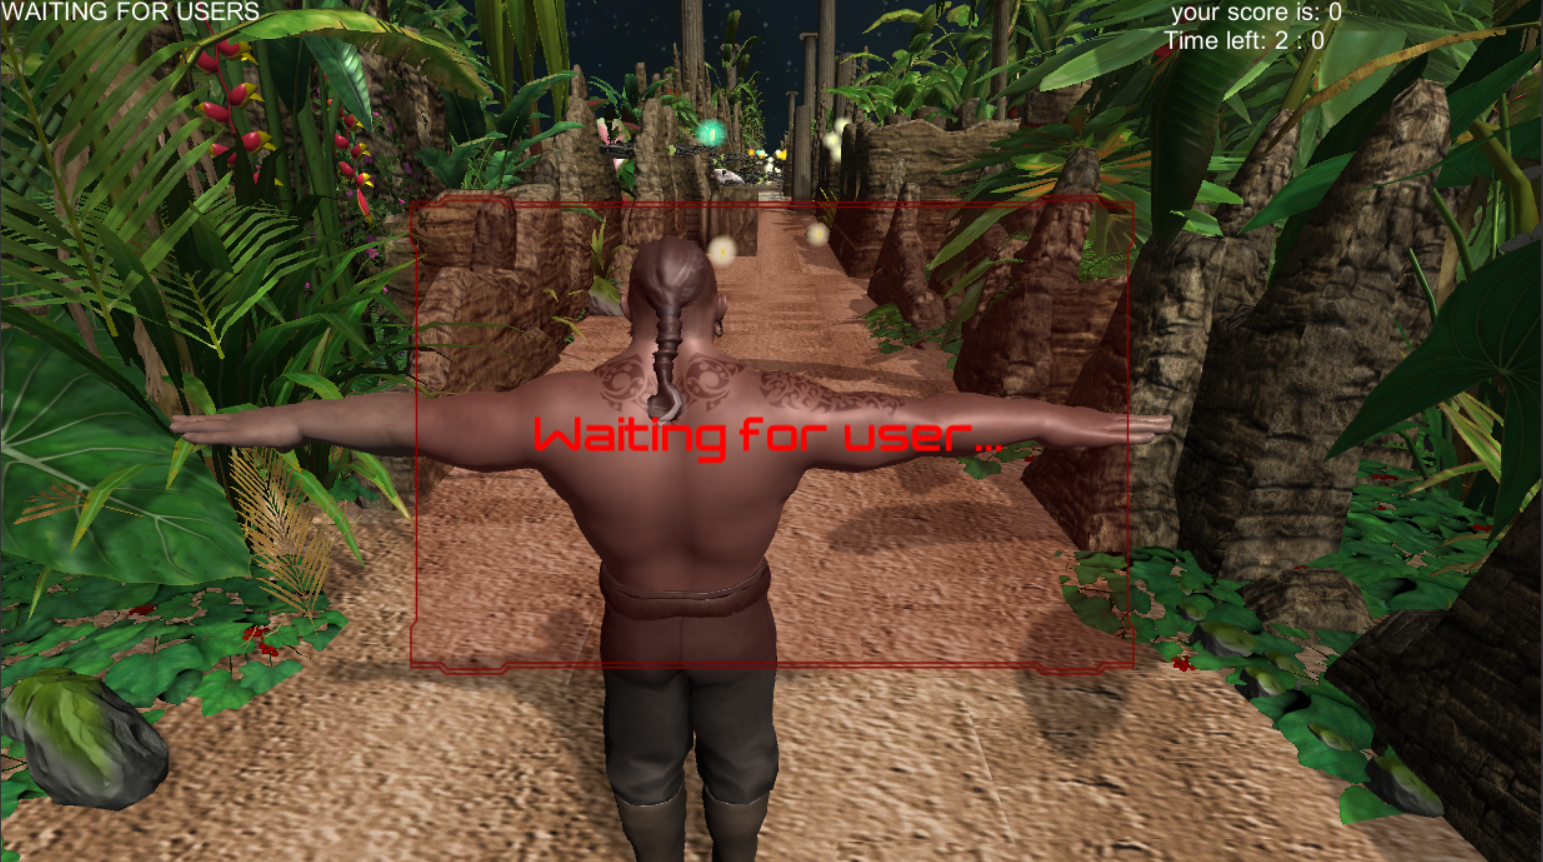
\includegraphics[width=\textwidth]{WaitingForUser}
    \caption{``Waiting for user'' popup screen.}
    \label{fig:witing}
\end{figure}
   
\paragraph{Help Menu}
The help menu, as presented in Figure \ref{fig:help} lets the user know how to interact with the game, change the speed of the game, and start or stop the game. The Back button allows the user to go back to the Home screen.\\ 
\begin{figure}[h]
    \centering
    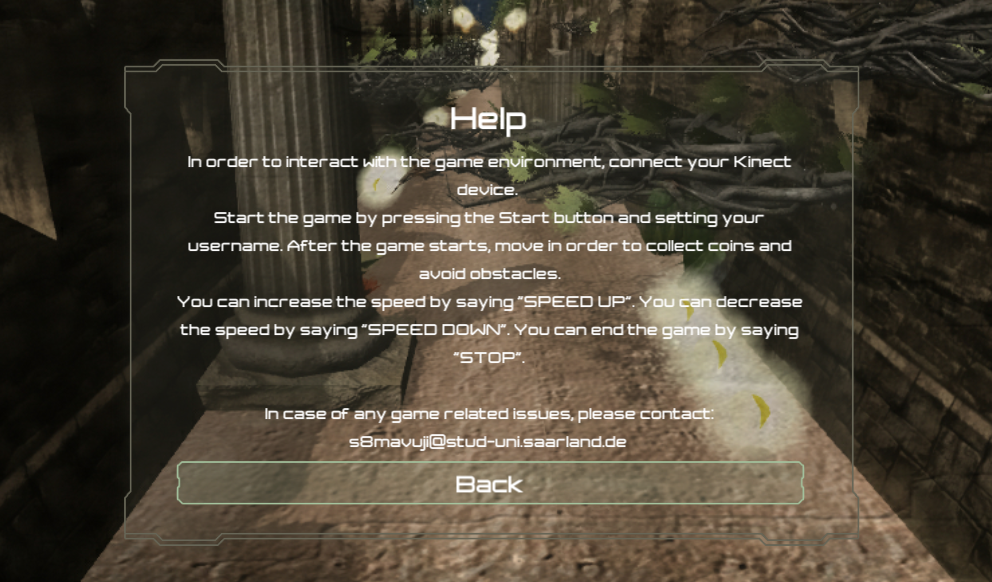
\includegraphics[width=\textwidth]{Help}
    \caption{Help menu.}
    \label{fig:help}
\end{figure}
\paragraph{Volume Menu}
The volume menu showed in Figure \ref{fig:volume}, gives users the possibility to modify the volume of the background music, sound effects (coins and obstacle collision sounds).
\begin{figure}[h]
    \centering
    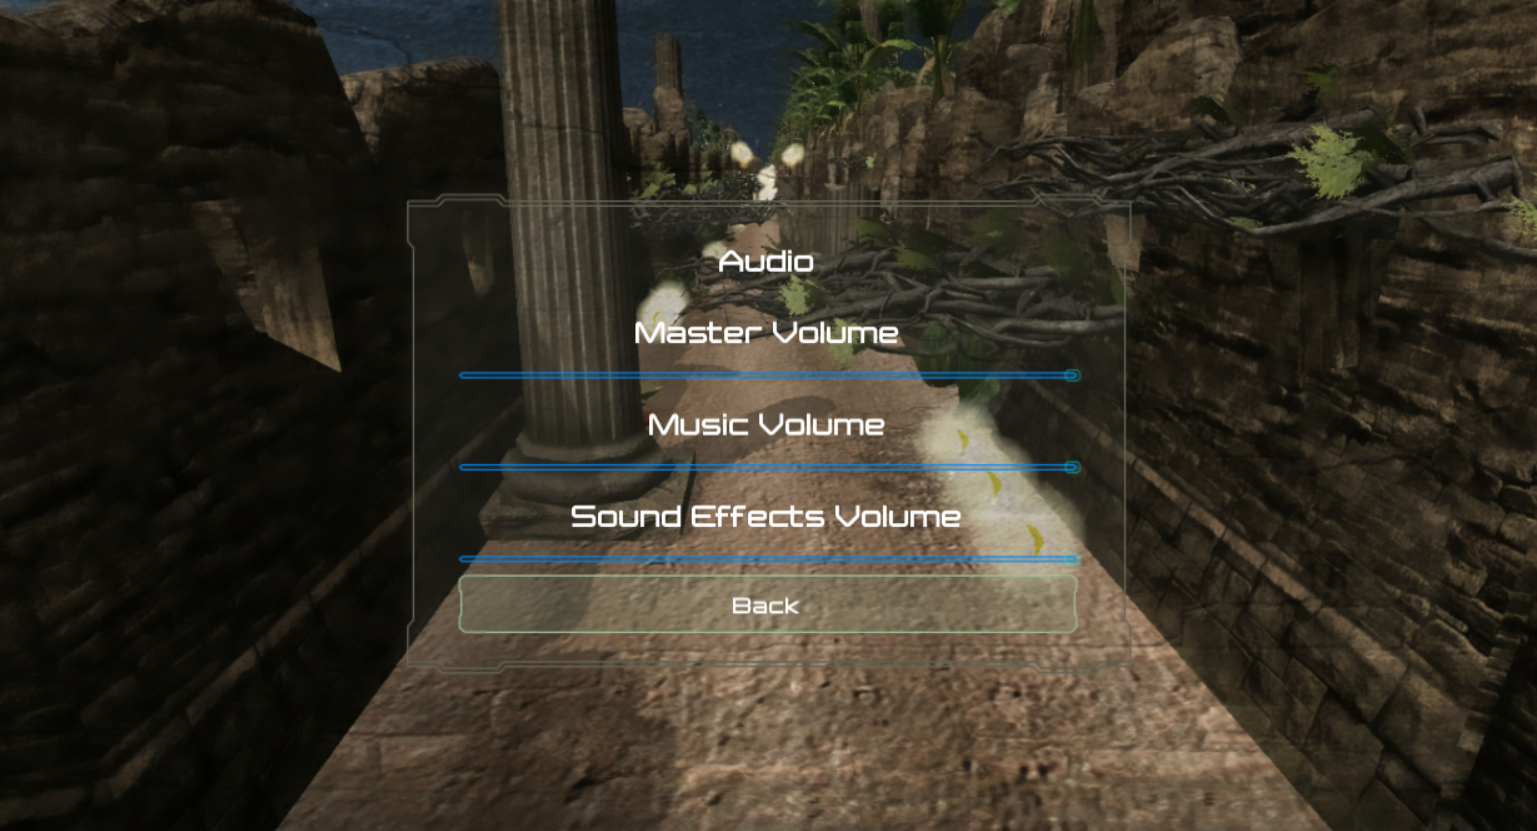
\includegraphics[width=\textwidth]{Volume}
    \caption{Adjust volume menu.}
    \label{fig:volume}
\end{figure}
\paragraph{High Score Menu}
The high score menu depicted in Figure \ref{fig:highscore} ranks the user who played the exergame based on the points collected during one gameplay. The leaderboard also displays the duration of the gameplay. This is a global highscore board. It is different than the one presented in Figure \ref{fig:individualScore} since it includes all the players and their scores. Contrarily, the individual score board, displays only the scores of the user who currently played the exergame. The Back button allows the user to go back to the Home screen.\\
\begin{figure}[h]
    \centering
    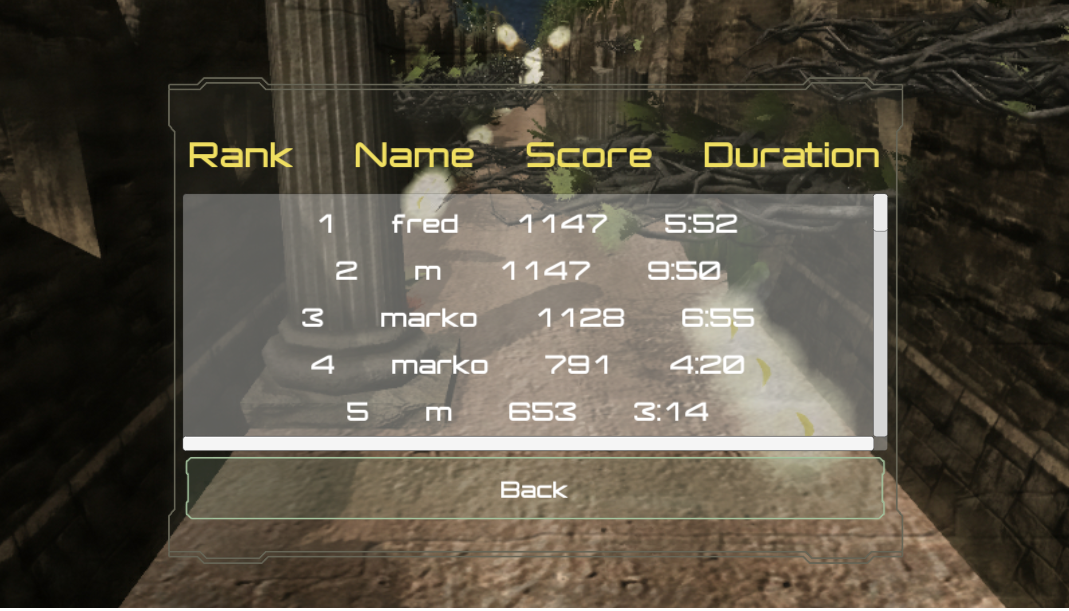
\includegraphics[width=\textwidth]{HighScore}
    \caption{High score menu.}
    \label{fig:highscore}
\end{figure}
\paragraph{Quit Menu}
The quit menu button exits the game. 
\section{Game Segments Overview}
Following recommendations from experts, available literature, and results from the first study, the list of warm up movements the users were required to perform during the game play has been updated. As already mentioned, each warm up movement the user was required to perform has been represented by a game segment. Additionally, we introduced so called \textit{filler} segments. In these segments no movements were required to be performed. Their only purpose was to give users a short amount of time to prepare for the subsequent game segment. By generating the segments randomly during gameplay, each game play was unique. Our main goal was to make the exergame intuitive to use. That is, the movements should come natural to the users and should not require further explanation. This was the result of our iterative and user centered design approach. We designed the segments based on the movements that can help users to warm up, and not contrarily. Figure \ref{fig:topview} gives an overview of all the segments used in the exergame. \\
\begin{figure}[h]
    \centering
    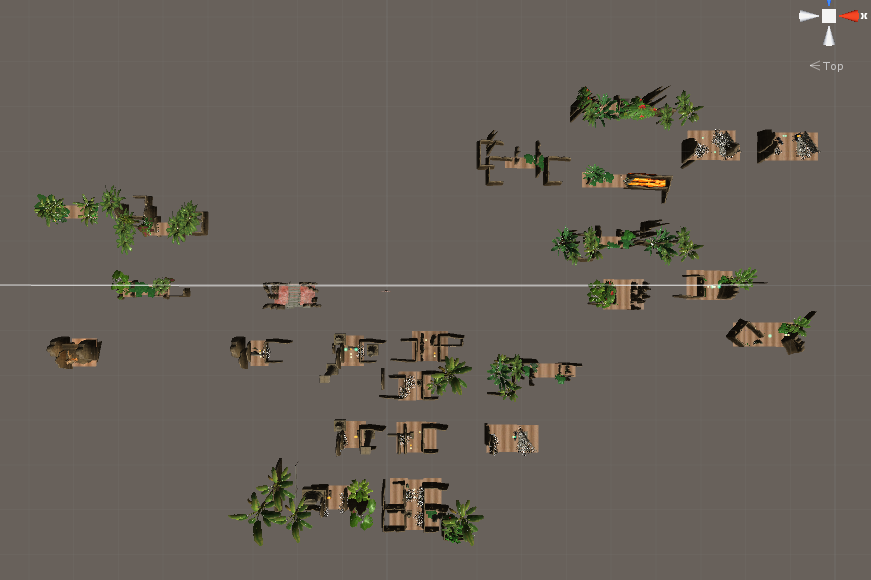
\includegraphics[width=0.9\textwidth]{SegmentsTopView}
    \caption{Overview of game segments - top view.}
    \label{fig:topview}
\end{figure}\\
In most of the segments depicted in Figure \ref{fig:topview}, one specific movement is required to be performed. Some segments are without obstacles and are present in order for the users to prepare for the next segment (and movements). Also, segments without any obstacles are used at the beginning of the exergame. At the very start, ten filler segments are generated, however this number has made adjustable. The empty segments are placed at the beginning in order to avoid any sudden movements by the player risking injuries. Moreover, not having to perform any movements gives the player time to adjust to the gameplay and prepare for the movements.\\\pagebreak Figure \ref{fig:wolfRight} shows the segment in which the user is required to move the hand in the upper position and, in the same time, avoid the \textit{wolf} obstacle. In case the user comes in contact with the wolf obstacle that is dynamic and is moving, the user is substracted one point from the overall score.\\
\begin{figure}[h]
    \centering
    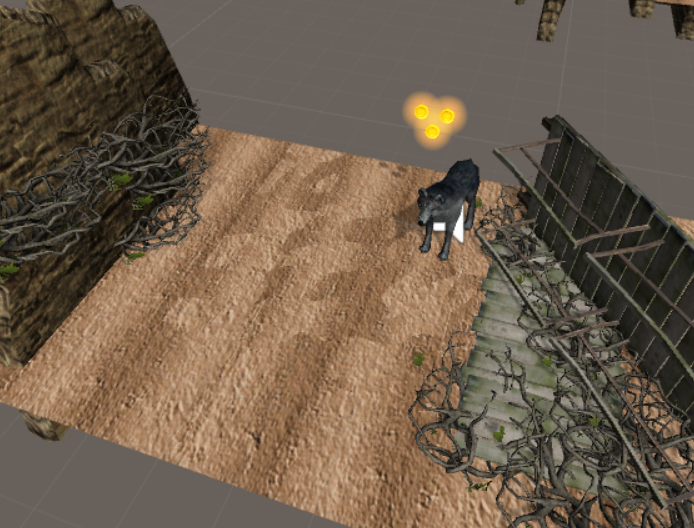
\includegraphics[width=0.8\textwidth]{HandUpRightWolf}
    \caption{Right hand up segment.}
    \label{fig:wolfRight}
\end{figure}\\
Figure \ref{fig:bridge} is one of the filler segments used for the users to prepare for the next movement. However, in case the user does not use the bridge and comes in contact with the walls or lava obstacles, the user is looses a point. \\
\begin{figure}[h]
    \centering
    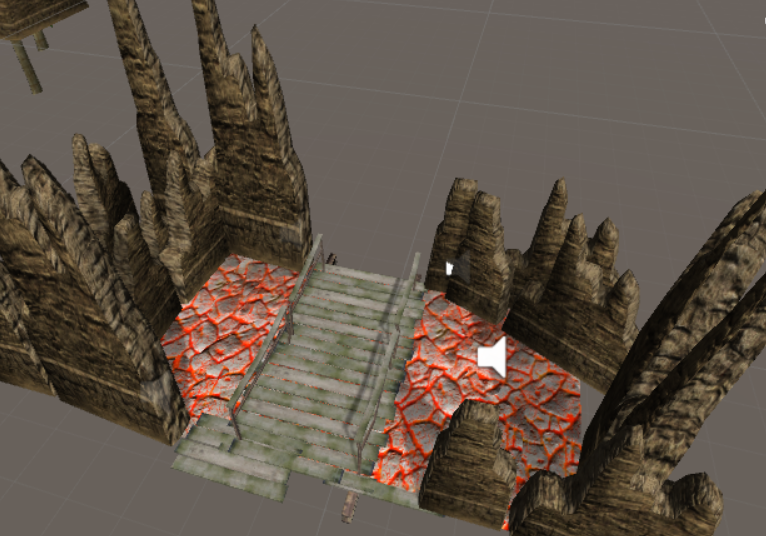
\includegraphics[width=0.8\textwidth]{Bridge}
    \caption{Bridge segment.}
    \label{fig:bridge}
\end{figure}\\
Figure \ref{fig:goblin} and \ref{fig:2wolfs} represent segments where  the user is given an option to chose which movement to perform. Both the movements include rising hand in the upper position. The decision is left to the user. In case the user opts for the left side, the possible reward is a \textit{blue coin} that is worth five points. However, there is a possibility to lose points by colliding with the obstacles. On the other hand, by choosing right side, the user can collect four coins without worrying about losing points.\\
\begin{figure}[h]
    \centering
    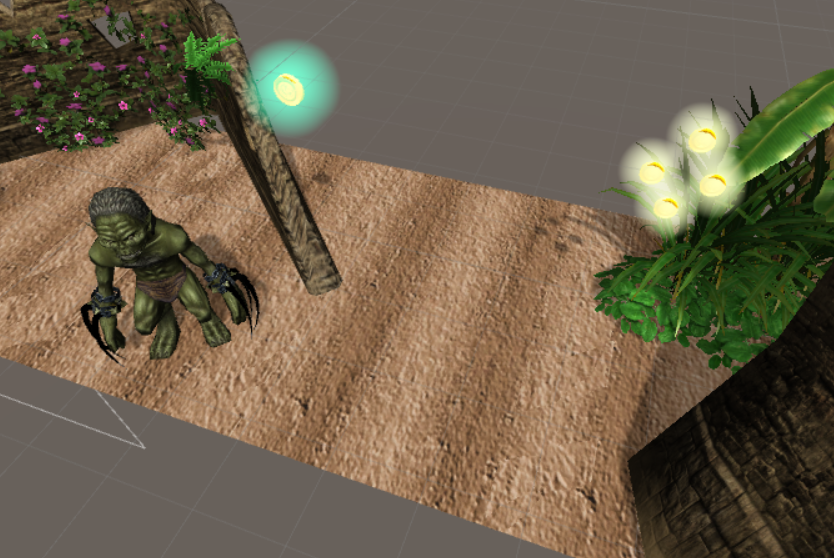
\includegraphics[width=0.8\textwidth]{GoblinHandLeftOrRight}
    \caption{Right or Left hand up segment.}
    \label{fig:goblin}
\end{figure}
\begin{figure}[h]
    \centering
    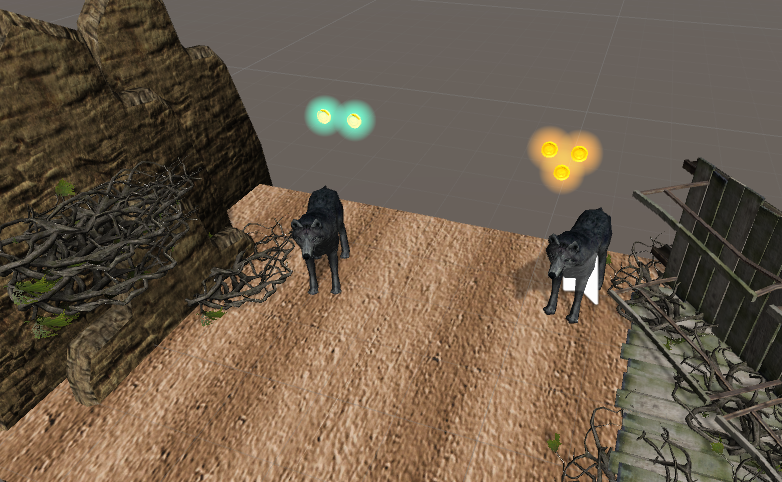
\includegraphics[width=0.8\textwidth]{2WolfsRight}
    \caption{Right or Left hand up segment.}
    \label{fig:2wolfs}
\end{figure}\\
Figure \ref{fig:star} depicts a game segment where the user was required to perform a \textit{star} jump in order to collect all the coins. \\
\begin{figure}[h]
    \centering
    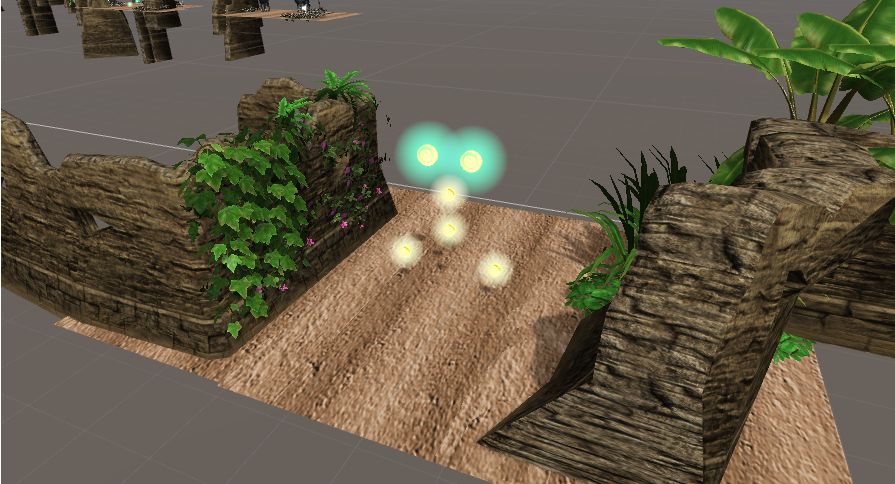
\includegraphics[width=0.8\textwidth]{JumpinJack}
    \caption{Star jump segment.}
    \label{fig:star}
\end{figure}\\
In Figure \ref{fig:jumpleft} and \ref{fig:jumpright} shows game segments where the user was required to perform jump to the left and jump to the right in order to avoid the obstacles. In case the user hit one of the obstacle, the overall user score was reduced by one.\\
\begin{figure}[h]
    \centering
    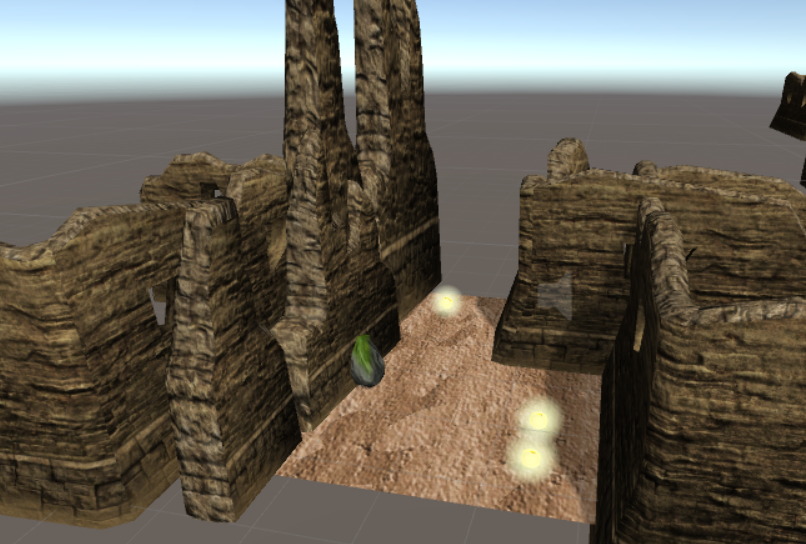
\includegraphics[width=0.9\textwidth]{JumpLeft}
    \caption{Jump left segment.}
    \label{fig:jumpleft}
\end{figure}
\begin{figure}[h]
    \centering
    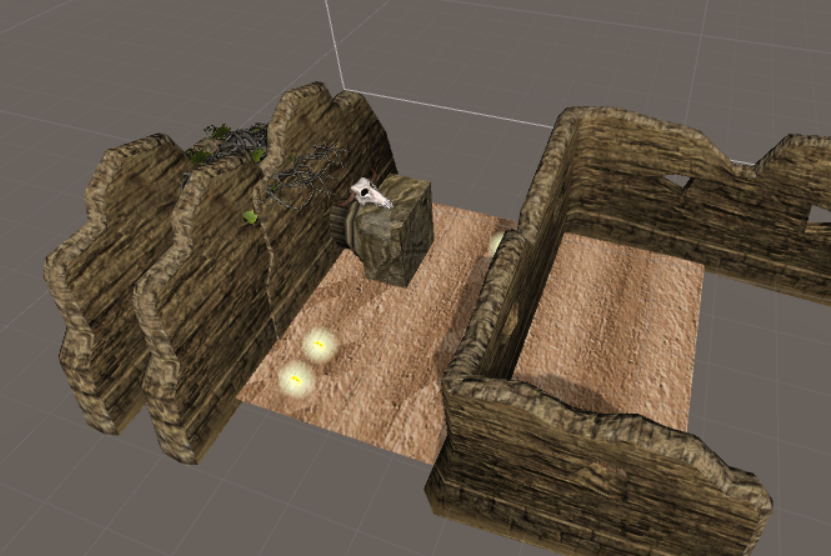
\includegraphics[width=0.9\textwidth]{JumpRight}
    \caption{Jump right segment.}
    \label{fig:jumpright}
\end{figure}\\
In the following Figure \ref{fig:jumpup}, the user was required to perform a jump in order to avoid the obstacle and collect the coins. The obstacle depicted was the lowest in the middle and would result in three collected coins in case performed correctly without colliding with the obstacle. In the meantime, the user is presented with a choice of collecting a coin the was worth four points. These coins were, however, placed in a position that required higher jump in order to be collected. There was also a higher chance to hit the obstacle since it was placed higher. \\
\begin{figure}[h]
    \centering
    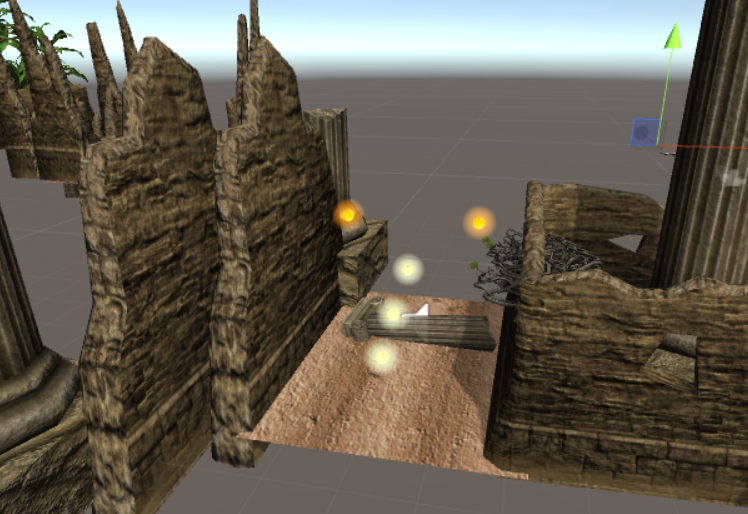
\includegraphics[width=0.9\textwidth]{JumpUp}
    \caption{Jump up segment.}
    \label{fig:jumpup}
\end{figure}\\
Figure \ref{fig:leftup} and \ref{fig:rightup} depict segments in which the user was required to perform a movement with the left and right arm in order to collect the coins. The obstacle was placed below the coins and one point is reduced from the user's overall score in case it was hit.\\
\begin{figure}[h]
    \centering
    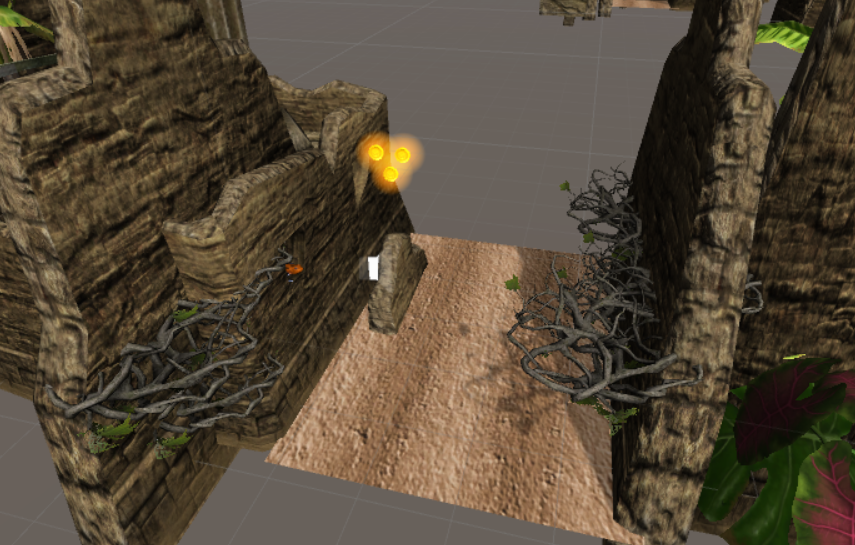
\includegraphics[width=0.9\textwidth]{LeftHandUp}
    \caption{Left hand up segment.}
    \label{fig:leftup}
\end{figure}
\begin{figure}[h]
    \centering
    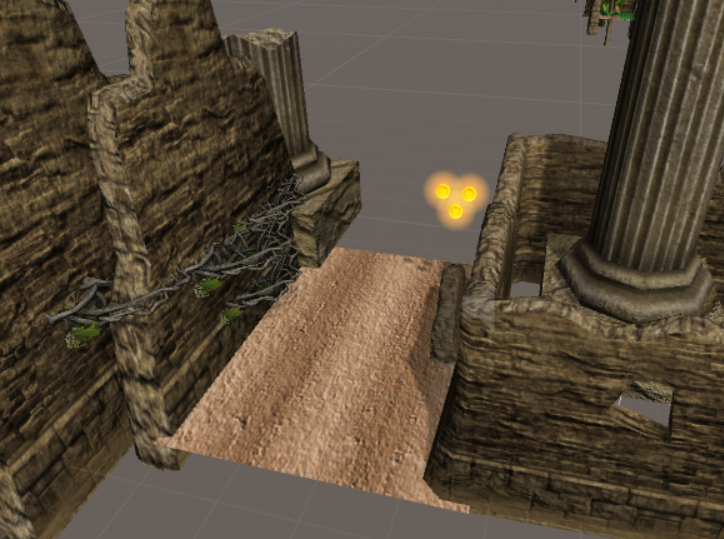
\includegraphics[width=0.9\textwidth]{RightHandUp}
    \caption{Right hand up segment.}
    \label{fig:rightup}
\end{figure}

Figure \ref{fig:squat} depicts a game segment in which the user was required to perform a squat and by doing that collect coins. In case the user hit the obstacles placed above the coins, the overall score was reduced by one.\\
\begin{figure}[h]
    \centering
    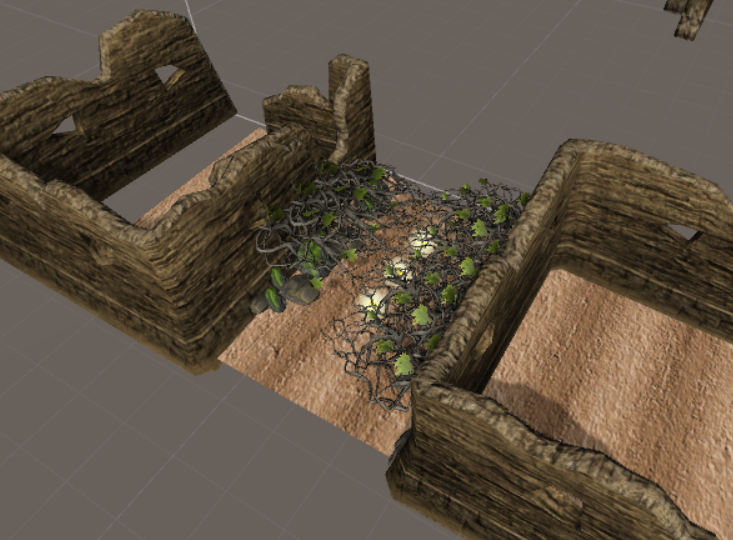
\includegraphics[width=0.9\textwidth]{Squat}
    \caption{Squat segment.}
    \label{fig:squat}
\end{figure}

In Figures \ref{fig:squatleft} and \ref{fig:squatright} the user was required to perform a jump left or right and perform a squat. As in previous segments, in case an obstacle was hit, the overall score was reduced by one.\\
\begin{figure}[h]
    \centering
    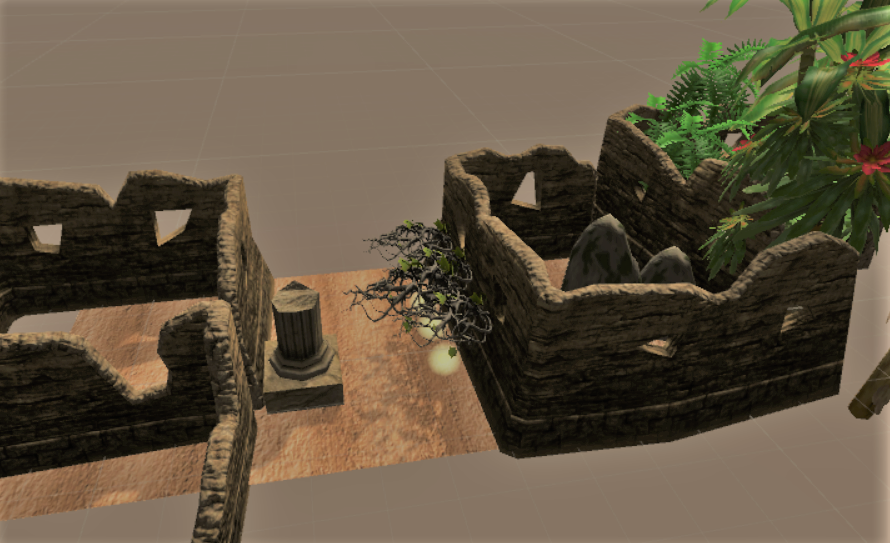
\includegraphics[width=0.9\textwidth]{SquatRight}
    \caption{Squat and move right segment.}
    \label{fig:squatright}
\end{figure}
\begin{figure}[h]
    \centering
    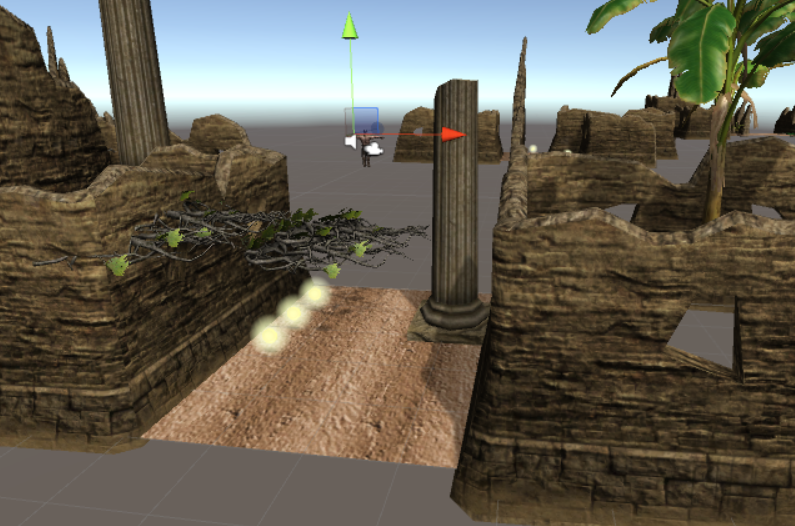
\includegraphics[width=0.9\textwidth]{SquatLeft}
    \caption{Squat and move left segment.}
    \label{fig:squatleft}
\end{figure}

The following figures depict the filler (empty) segments that are placed at the beginning of the game and in between segments with obstacles.

\begin{figure}[h]
    \centering
    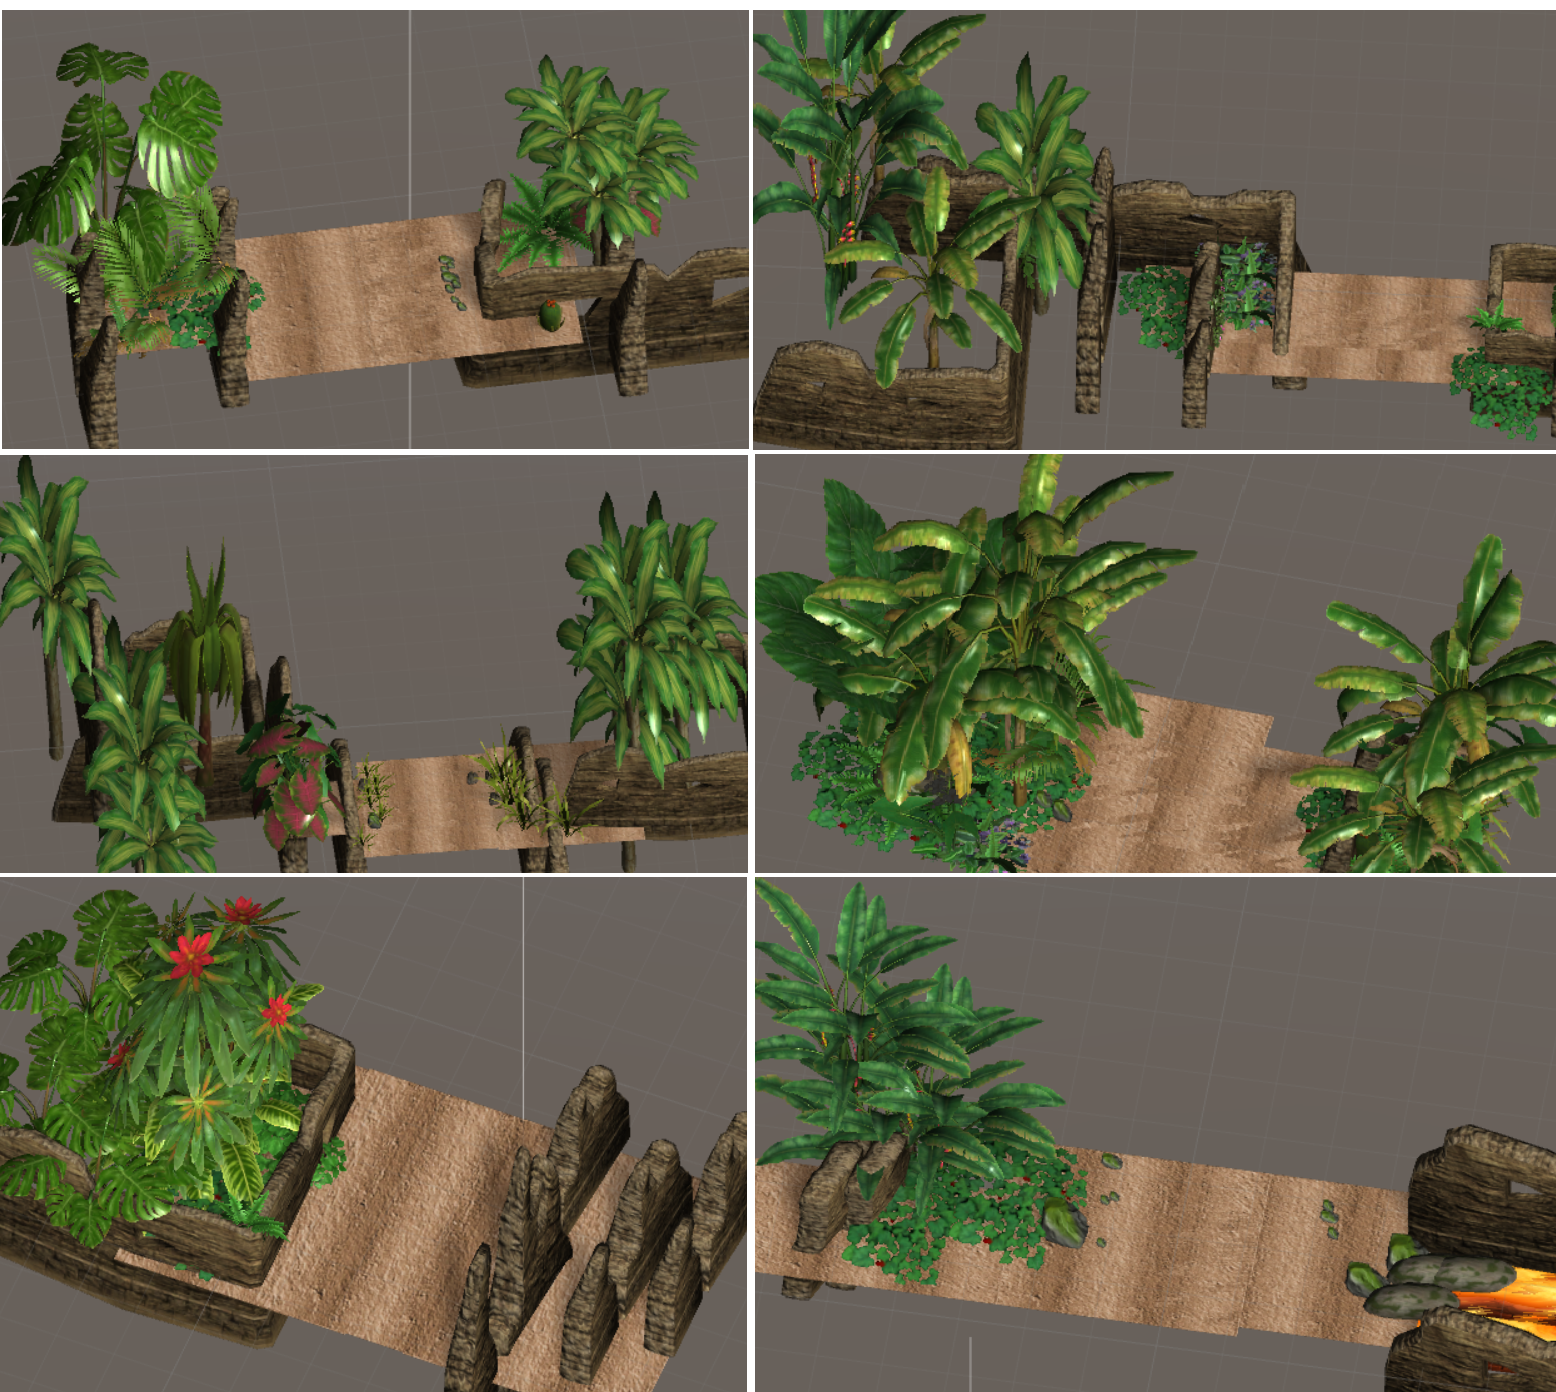
\includegraphics[width=\textwidth]{Filler1}
    \caption{Filler segments.}
    \label{fig:filler}
\end{figure}

\section{Game End Overview}
\label{endgamelabel}


\begin{figure}[h]
    \centering
    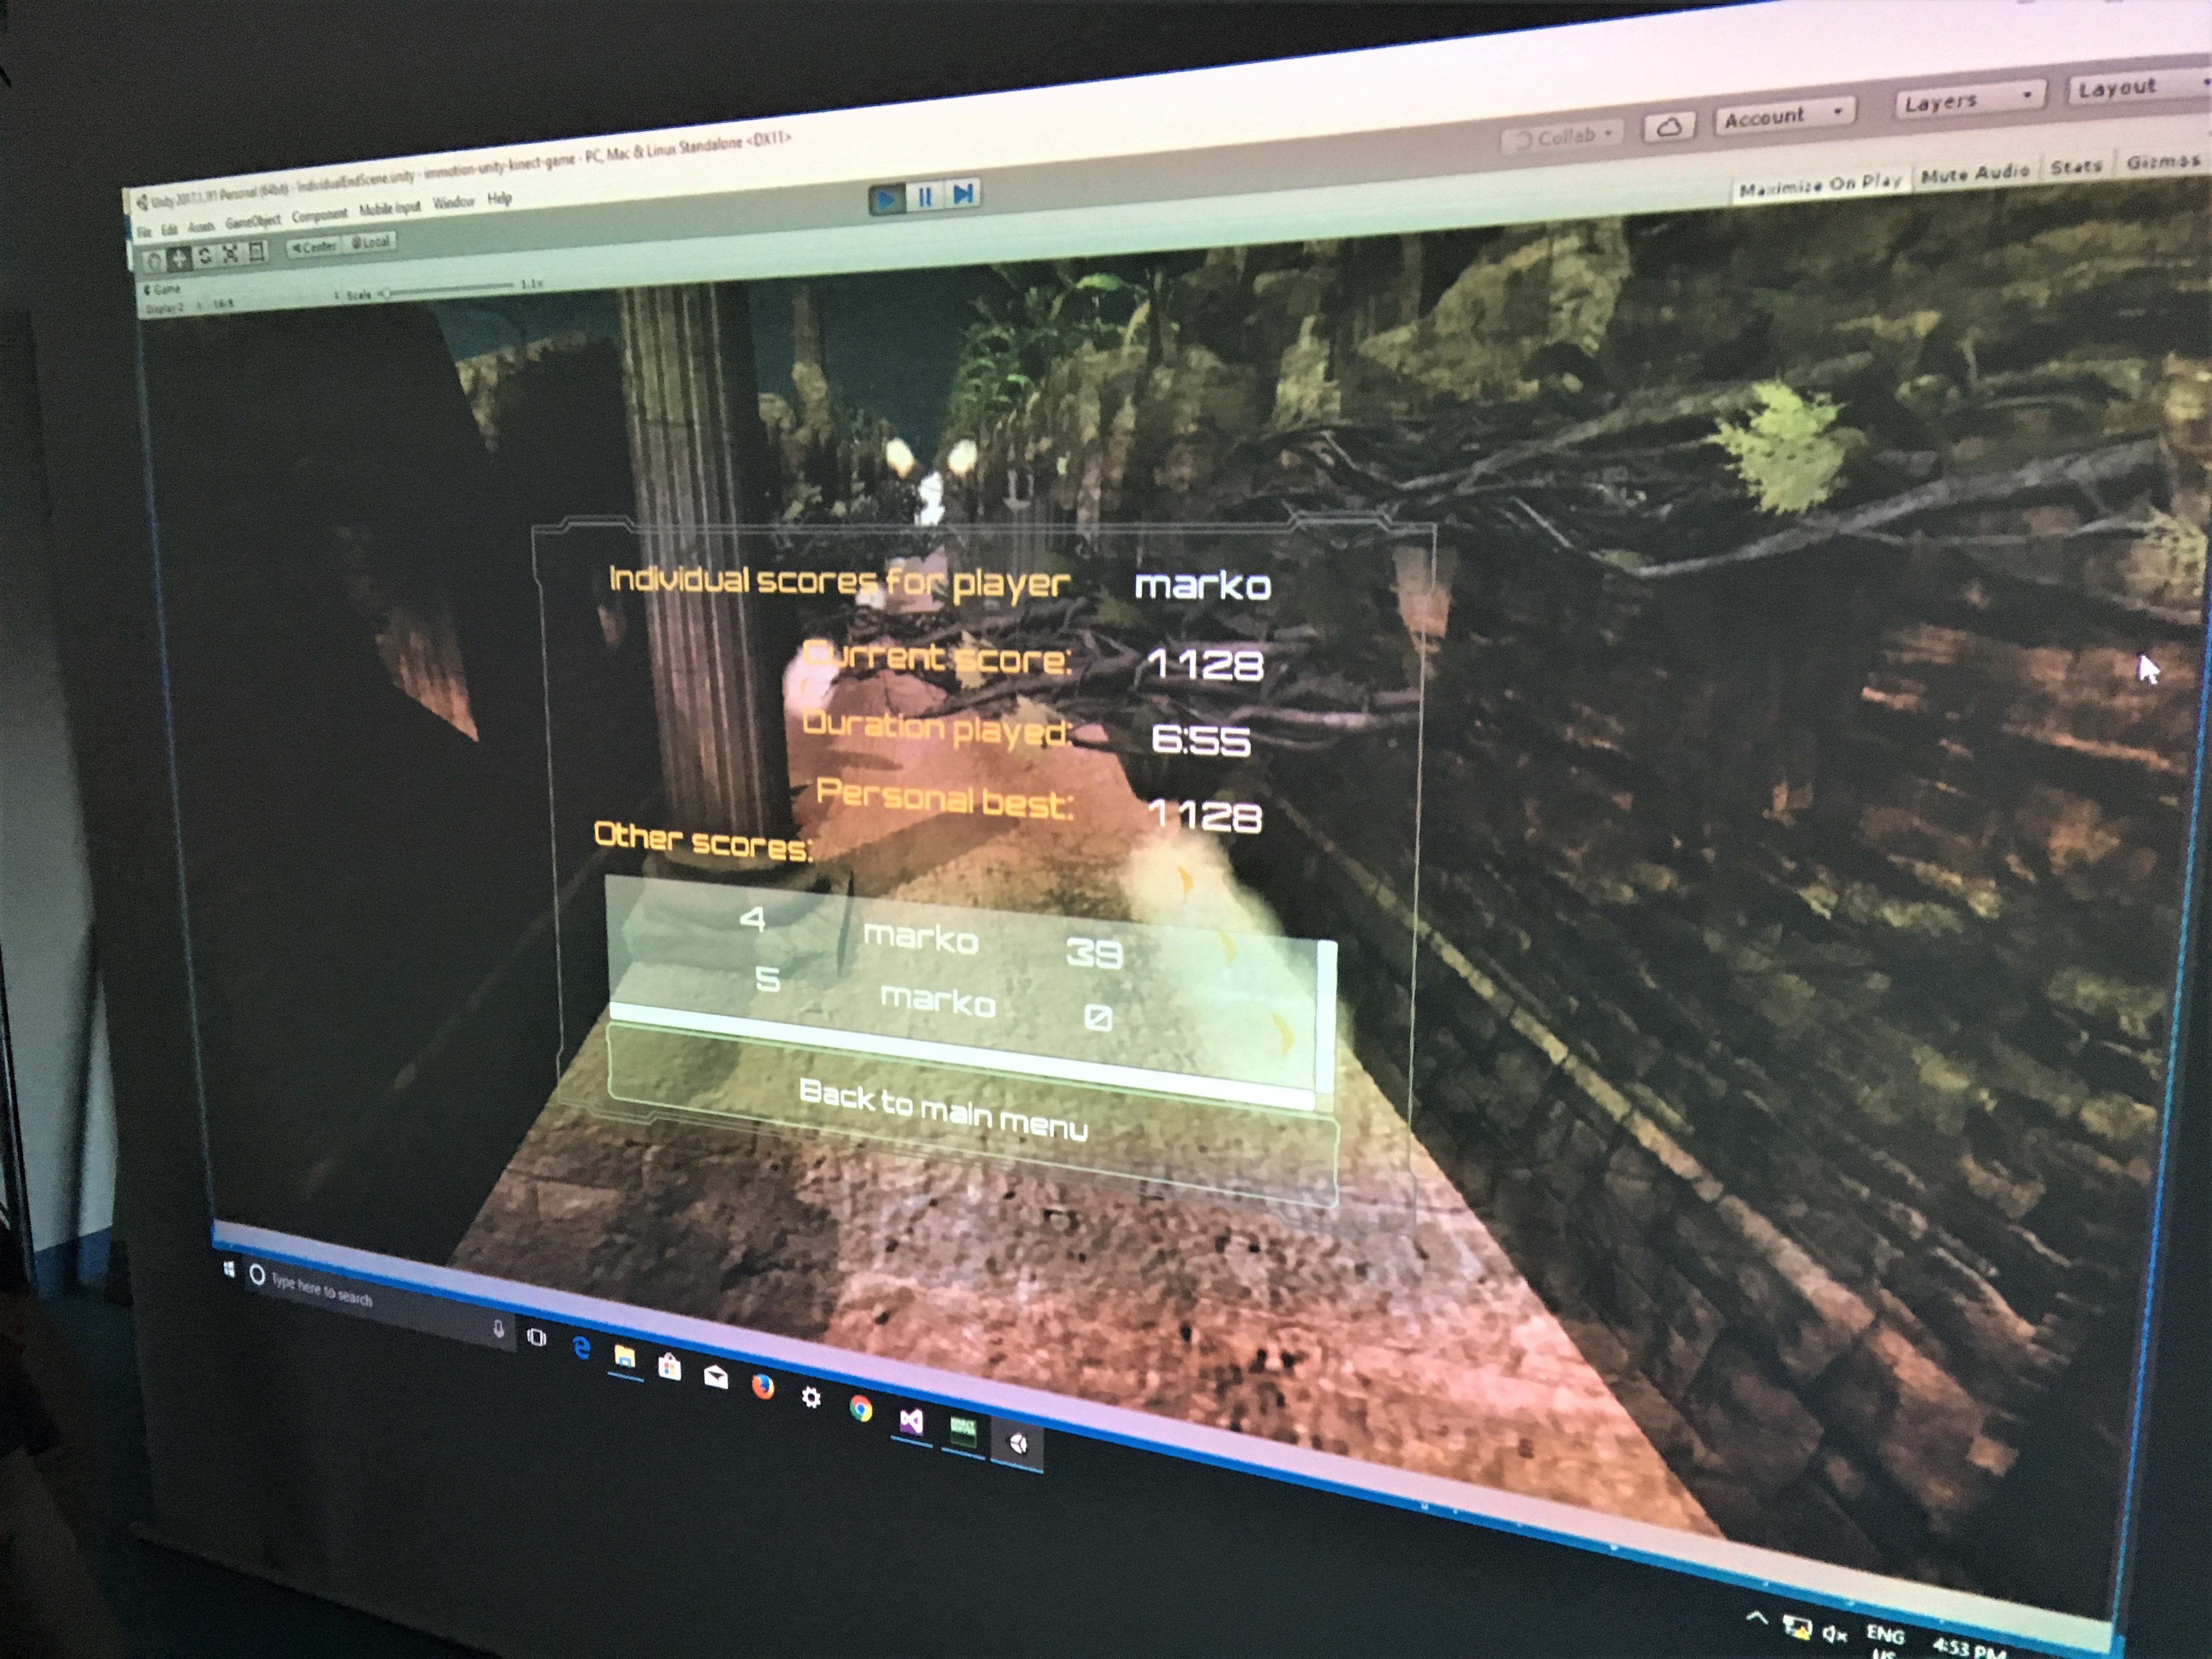
\includegraphics[width=\textwidth]{individualScore}
    \caption{Individual scores menu.}
    \label{fig:individualScore}
\end{figure}
